%%%%%%%%%%%%%%%%%%%%%%%%%%%%%%%%%%%%%%%%%%%%%%%%%%%%%%%%%%%%%%%%%%%%%%%%%%%%%%%%
\chapter*{Приложение}							% Заголовок
\addcontentsline{toc}{chapter}{Приложение}		% Добавляем его в оглавление

\begin{figure}[h]
  \center{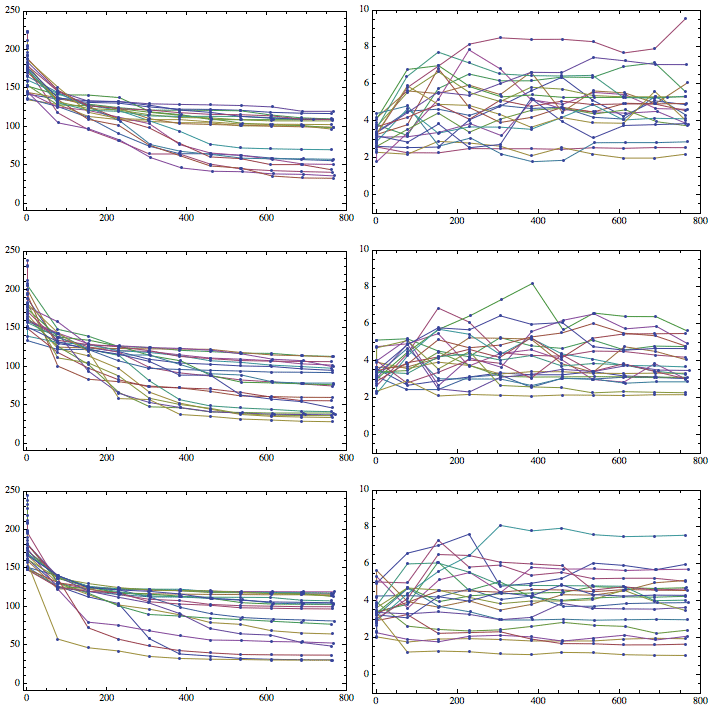
\includegraphics[width=17cm]{pm1}}
  \caption{Модель 1. $population\_size = 150, es\_lambda = 2,15,45$. 20 запусков}
  \label{img:pm1}
\end{figure}

\begin{figure}[h]
  \center{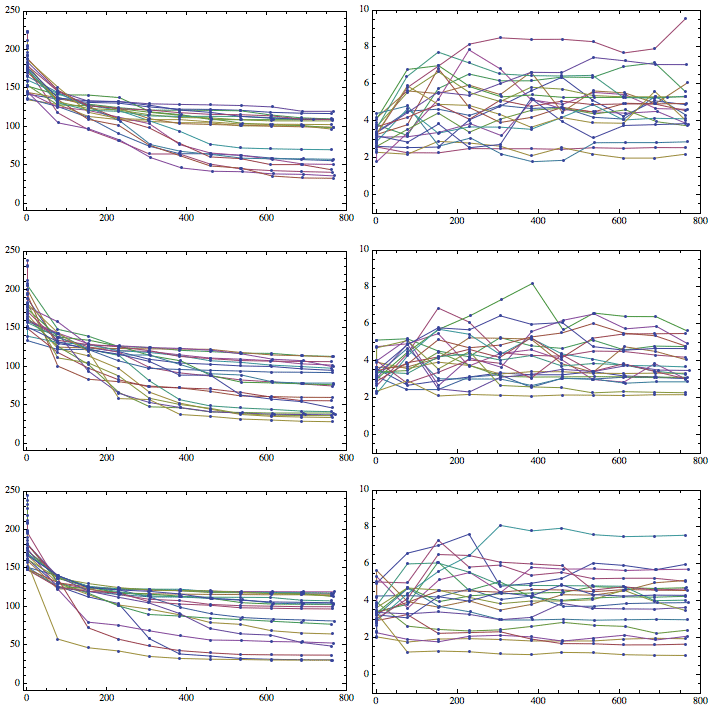
\includegraphics[width=17cm]{pm1}}
  \caption{Модель 2. $population\_size = 150, es\_lambda = 2,15,45$. 20 запусков}
  \label{img:pm2}
\end{figure}

\begin{figure}[h]
  \center{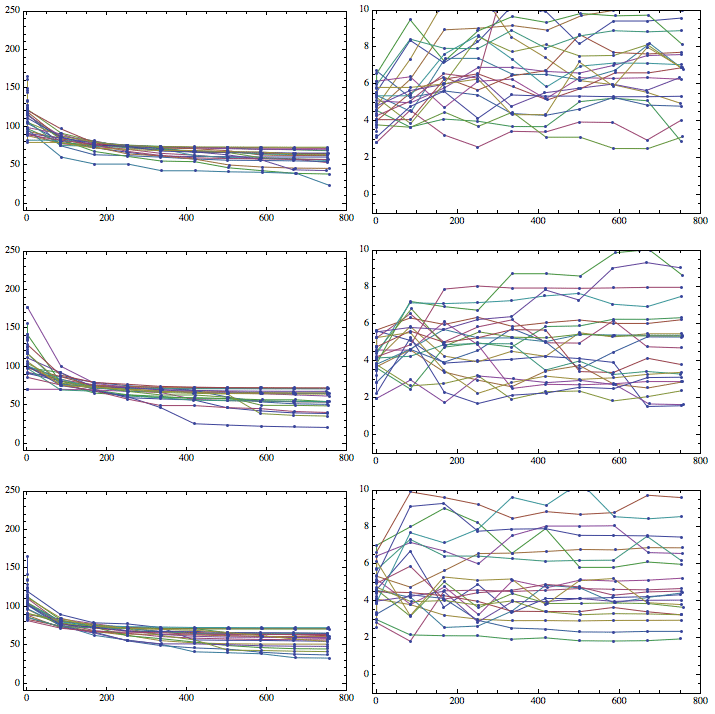
\includegraphics[width=17cm]{pm2}}
  \caption{Модель 3. $population\_size = 150, es\_lambda = 2,15,45$. 20 запусков}
  \label{img:pm3}
\end{figure}

\begin{figure}[h]
  \center{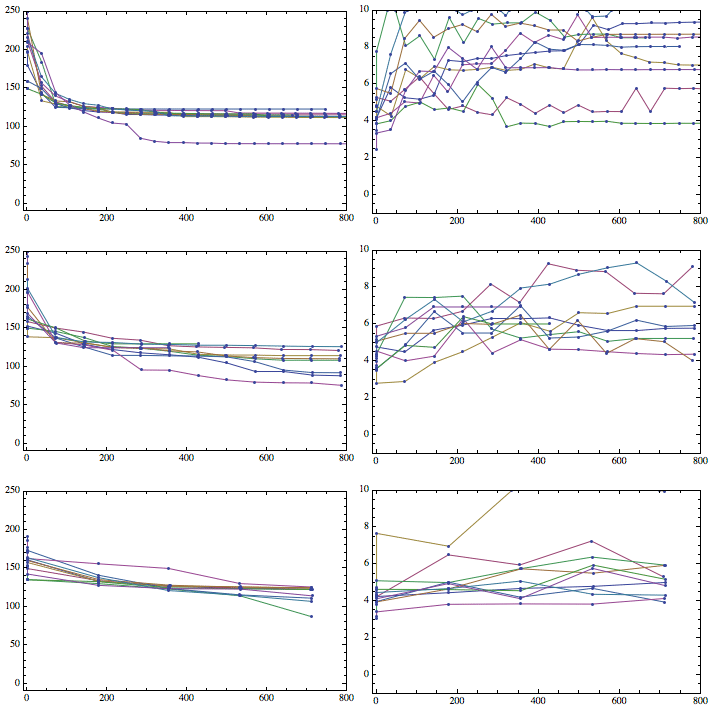
\includegraphics[width=17cm]{em1}}
  \caption{Модель 1. $population\_size = 70,140,350, es\_lambda = 6,10,30$. 10 запусков}
  \label{img:em1}
\end{figure}

\begin{figure}[h]
  \center{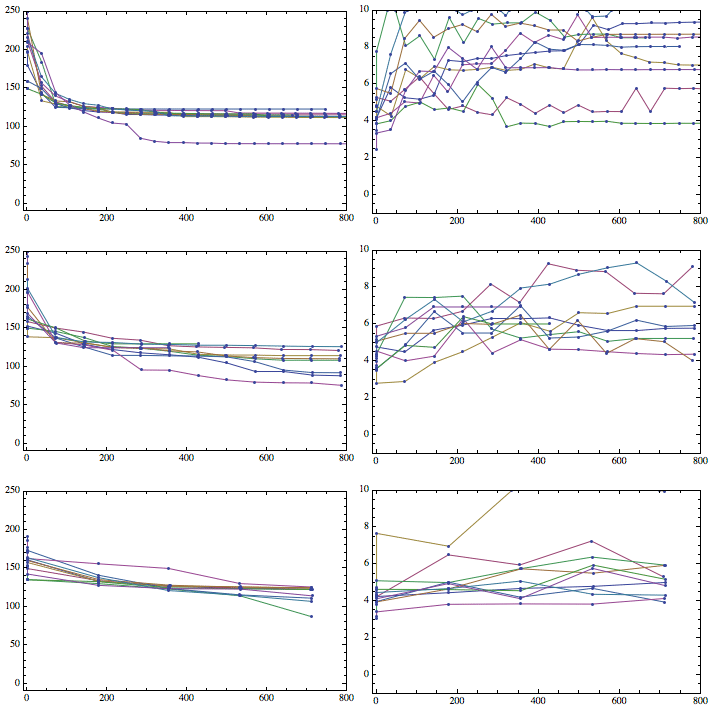
\includegraphics[width=17cm]{em1}}
  \caption{Модель 2. $population\_size = 70,140,350, es\_lambda = 6,10,30$. 10 запусков}
  \label{img:em2}
\end{figure}

\begin{figure}[h]
  \center{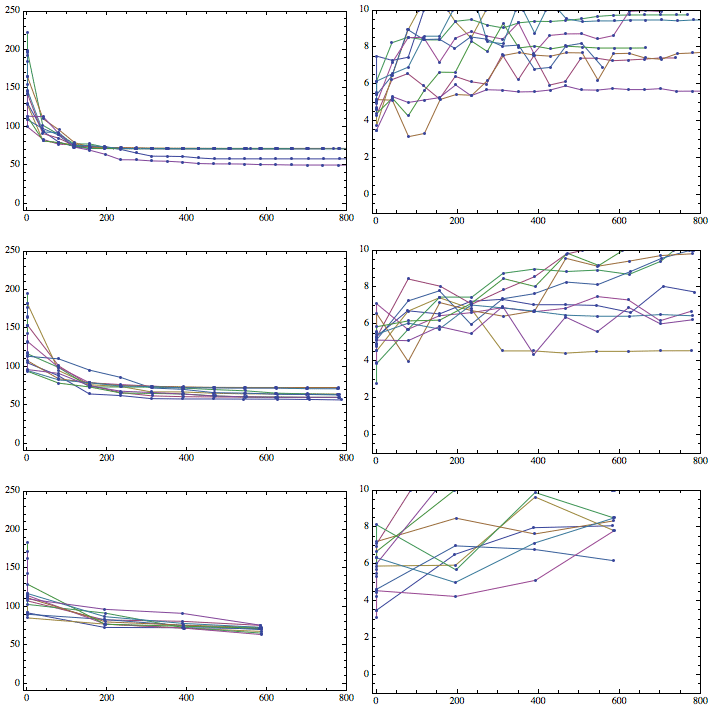
\includegraphics[width=17cm]{em2}}
  \caption{Модель 3. $population\_size = 70,140,350, es\_lambda = 6,10,30$. 10 запусков}
  \label{img:em3}
\end{figure}

\clearpage
%%%%%%%%%%%%%%%%%%%%%%%%%%%%%%%%%%%%%%%%%%%%%%%%%%%%%%%%%%%%%%%%%%%%%%%%%%%%%%%%
